
El proceso de cálculo que se va a seguir para la estimación completa de la instalación fotovoltaica conectada a red es el que se detalla en el libro de Óscar Perpiñán, tutor de este trabajo, denominado Energía Solar Fotovoltaica \cite{esf_book}. También se harán menciones a las presentaciones que se encuentran en el mismo enlace que el libro.\\

A lo largo de este capítulo, se utilizará el término \textbf{aplicación} para referirse a todo el conjunto de código relacionado tanto con proceso de obtención de todos los datos necesario como el de mostrar la información relevante al usuario.

\section{Obtención de datos del usuario}
Como se ha mencionado anteriormente, el objetivo principal de la aplicación es de realizar todos los cálculos que se necesitan para estimar una instalación fotovoltaica conectada a red, de la manera mas exacta posible,  en un emplazamiento concreto elegido por el usuario. Por tanto, el primer paso que tuve que dar con la aplicación fue la de obtener todos los datos necesarios para realizar dichos cálculos.
Estos datos son:
\begin{itemize}
\item Emplazamiento del usuario
\item Área, inclinación, orientación y nivel de suciedad de la superficie de instalación
\end{itemize}
\subsection{Emplazamiento del usuario}
Mas adelante, para poder obtener los datos de irradiación global en el plano horizontal, se necesitan los datos de latitud y longitud del sitio del que se quieren obtener dichos datos. Sin embargo, es poco intuitivo pedirle a un usuario que introduzca sus coordenadas, dado que la mayoría desconocen dichos datos.\\
Por lo tanto, la ruta que he tomado es la de pedirle al usuario su dirección, o una dirección cercana a su localización, y utilizar la API de Google Maps \footnote{\textit{API Google Maps}: Enlace interactivo al que se le pueden enviar los datos de una dirección y devuelve las coordenadas de latitud y longitud de un emplazamiento.  } para convertir dicha dirección en las coordenadas de latitud y longitud que necesito para poder extraer la irradiación que he mencionado antes.\\

Este proceso comienza por recoger los datos de la dirección, municipio y código postal a través del formulario que aparece en la página web.

Estos datos son recogidos en el código a través de un nombre único que han recibido:\\
\begin{lstlisting}[style=ES6, caption={Variables correspondientes a los tres campos}]
const addressInput = document.querySelector('#address');
const cityInput = document.querySelector('#city');
const postalInput = document.querySelector('#postal');
\end{lstlisting}

Una vez que tenemos estos datos recogidos en las variables, podemos pedir a la API de Google Maps las coordenadas de latitud y longitud de dicho emplazamiento encadenando las tres variables y una clave única de identificación,  para obtener un enlace único que se corresponde a dicha localización.\\

\begin{lstlisting}[style=ES6, label={lst:getCoordinates}, caption={Función encargada de solicitar los datos a la API}]
const getCoordinates = async () => {
	const address = addressInput.value.split(' ').join('+');
	const city = cityInput.value;
	const postal = postalInput.value;
	const requestURL = `${googleEndpoint}address=${address},${city},${postal}
										,spain&key=${googleApiKey}`;
	const response = await fetch(requestURL);
	const data = await response.json();
	const info = {
		formattedAdress: data.results[0].formatted_address,
		lat: data.results[0].geometry.location.lat,
		long: data.results[0].geometry.location.lng
	};

	return info;
};
\end{lstlisting}

La función de \textbf{getCoordinates} (\ref{lst:getCoordinates}) recoge el valor de la dirección y reemplaza los espacios con el signo + (formato requerido por la API) y lo concatena con el valor del campo de la ciudad y el código postal. Al final le añade una clave única que identifica la aplicación a la hora de establecer limites de uso y evitar abuso de la API.\\

Una vez creado este enlace único, el código lanza la petición al servicio y retorna con la información que es recogida y se guarda en dos variables \textbf{lat} y \textbf{long} para ser utilizadas posteriormente, a la hora de obtener los datos de irradiación global.

\subsection{Área, inclinación, orientación y nivel de suciedad de la superficie de instalación}

Además de las información de latitud y longitud del emplazamiento, el cálculo de la instalación también requiere de información relacionada con el área, la inclinación, la orientación y el nivel de suciedad de la superficie donde se va a realizar la instalación, para poder realizar una estimación lo mas exacta posible.

Estos valores son recogidos directamente de los campos de la pagina web, al igual que los campos anteriores, sin necesitar ningún trato especial:\\
\begin{lstlisting}[style=ES6, caption={Variables correspondientes a los campos indicados}]
const slope = document.querySelector('#slope');
const area = document.querySelector('#area');
const orientation = document.querySelector('#orientation');
const dirtLevel = document.querySelector('#dirt-level');
\end{lstlisting}

\section{Obtención de la irradiación global media en el plano horizontal}
\label{section:get_global_rad}

El primer paso del cálculo de una instalación fotovoltaica es el de conocer la irradiación global media en el plano horizontal para el emplazamiento donde se va a realizar el cálculo. En la sección anterior se obtuvieron las coordenadas de latitud y longitud del emplazamiento introducido por el usuario.\\

En esta sección, se va a obtener la irradiación para las dichas coordenadas utilizando un servicio de ADRASE \footnote{\textit{ADRASE}: Acceso a Datos de irradiación Solar en España \url{http://www.adrase.com/}}, un proyecto realizado por el CIEMAT. Este servicio ofrece de manera gratuita y de uso libre, datos correspondientes a valores medios mensuales de irradiación global en el plano horizontal para toda la geografía española.\\

Los datos están disponibles a través de un mapa interactivo y de unos enlaces personalizados que incluyen la valores de latitud y longitud para los que se desea obtener dicha información. En esos enlaces se ofrecen los datos de irradiación global mínima, media y máxima en el plano horizontal.\\

Con el objetivo de no saturar la pagina de ADRASE y evitar error de funcionamiento de la aplicación debidos a la posibilidad de que la página desaparezca en un futuro, se ha realizado una descarga de los datos de la página, con un intervalo de 0.1 tanto en longitud como en latitud y se han guardado en una base de datos.De esta forma también se reducen los tiempos de cálculo en gran medida al tener un acceso casi instantáneo a los valores medios de irradiación. 
Una explicación detallada de como se ha realizado dicha descarga se incluye en el Anexo. ( ** TO DO Anexo con explicación **).
\newpage

\section{Naturaleza de la radiación solar}

\subsection{Radiación fuera de la atmósfera terrestre}
\label{section:extra-irrad}
La radiación emitida por el Sol atraviesa el espacio vacío en todas las dirección sin sufrir pérdidas a causa de la interacción con los medios material. Sin embargo, la irradiancia solar, que se define como la densidad de flujo radiante solar, se ve atenuada por el cuadrado de la distancia. Parte de esta irradiancia es interceptada por la Tierra. Dada la relación entre la distancia con el Sol y el tamaño de nuestro planeta, se puede asumir que su valor es constante en toda la superficie exterior de la atmósfera. El valor promedio de esta irradiancia, según varias campañas de medición es de $B_{0} = 1367 \frac{W}{m^2}$.

Para calcular la irradiancia incidente en una superficie tangente a la atmosfera en una latitud, debemos tener en cuenta que la distancia entre la Tierra y el Sol varía a lo largo del año, debido a la excentricidad de la órbita elíptica que describe nuestro planeta. La ecuación para calcular dicho valor es:\\
\begin{equation}\label{eqn:B00}
B_0(0) = B_0\epsilon_0\cos\theta_{zs}
\end{equation}\\


Es importante resaltar que el valor de la irradiancia extra-atmosférica o extra-terrestre solo requiere consideraciones atmosféricas. Así, integrando la ecuación \ref{eqn:B00}, podemos calcular la irradiación diaria extra-terrestre con la ecuación obtenida:\\
\begin{equation}\label{eqn:B0d0}
B_{0d}(0)=-\frac{T}{\pi}B_0\epsilon_0·(\omega_s\sin\phi\sin\delta + \cos\phi\cos\delta\sin\omega_s)
\end{equation}\\

Es posible demostrar que el promedio mensual de esta irradiación diaria coincide numéricamente con el valor de irradiación diaria correspondiente a los denominados días promedios, días en los que la declinación correspondiente coincide con el promedio mensual. Por tanto, podemos calcular el valor medio mensual de la irradiación diaria extra-atmosférica con el valor de la declinación de uno de los doce días promedio.

Estos doce días promedios son:

\begin{table}[ht]
\label{tab:dias_promedio}
\centering
\begin{tabular}{|l|l|l|l|l|l|l|l|l|l|l|l|l|}
\hline
Mes   & Ene & Feb & Mar & Abr & May & Jun & Jul & Ago & Sep & Oct & Nov & Dic \\ \hline
$d_n$ & 17  & 45  & 74  & 105  & 135  & 161  & 199  & 230  & 261  & 292  & 322 & 347  \\ \hline
\end{tabular}
\caption{Dias promedio}
\end{table}

Para calcular esta irradiación diaria, debemos calcular primero los diferentes componentes que forman parte de esta:
\begin{itemize}
\item $B_{0} = 1367 \frac{W}{m^2}$
\item Factor de corrección por excentricidad: $\epsilon_0 = 1 + 0,033 \cdot \cos(\frac{2\pid_n}{365})$

En código se representa de la siguiente manera:
\begin{lstlisting}[style=ES6, caption={Factor de corrección por excentricidad}]
		const exct = 1 + 0.033 * Math.cos((2 * Math.PI * elem.normalDay) / 365)
\end{lstlisting}
\item Ecuación de Cooper para la declinación: $\delta = 23,45\deg · \sin(\frac{2\pi·(d_n+284)}{365})$

En código se representa de la siguiente manera:
\begin{lstlisting}[style=ES6, caption={Ecuación de Cooper para declinación}]
		const decl = 23.45 * Math.sin((2 * Math.PI * (elem.normalDay + 284)) / 365)
\end{lstlisting}
\item Cenit Solar: $\cos(\theta_{zs}) = \cos(\delta)\cos(\omega)\cos(\phi) + \sin(\delta)sin(\phi)$\\

Para el calculo del cenit solar, hay que tener en cuenta que varía en función de la hora del día, así que se deberá calcular un valor para cada una de las 24h del día, con la diferencia de que en el cálculo, las horas irán de -12 a 12 en lugar de 0 a 23 y además, tendremos que convertir las horas a ángulos multiplicando por 15$\deg$. De tal manera, que en código, el calculo del cenit solar, tendrá ésta representación:\\
\begin{lstlisting}[style=ES6, caption={Cálculo del cenit solar}]
		for (let h = -12; h < 12; h++) {
			const cosZenit =
				Math.cos(deg2rad(elem.decl)) * Math.cos(deg2rad(h * 15)) * 	
					  Math.cos(deg2rad(newData.latitude)) +
				Math.sin(deg2rad(elem.decl)) * Math.sin(deg2rad(newData.latitude))
			const zenitVal = rad2deg(Math.acos(cosZenit))
		}
\end{lstlisting}
\end{itemize}

Aplicando estos cálculos a la ecuación \ref{eqn:B0d0} podemos calcular el valor de la irradiancia extra-terrestre diaria $B_{0d}(0)$ con la siguiente expresión:
\begin{lstlisting}[style=ES6, caption={Equación para B0d0}]
		const B0d0 =
			-(24 / Math.PI) *
			B0 *
			elem.exct *
			(elem.ws * Math.sin(deg2rad(newData.latitude)) * Math.sin(deg2rad(elem.decl)) +
				Math.cos(deg2rad(elem.decl)) * Math.cos(deg2rad(newData.latitude)) * 
				Math.sin(elem.ws))
\end{lstlisting}
donde:
\begin{itemize}
\item B0: valor contante de 1367 $W/m^2$
\item exct: excentricidad
\item ws: ángulo amanecer
\item decl: declinación
\end{itemize}
Para el cálculo de la irradiancia solar que finalmente incide en una superficie localizada en la corteza terrestre será útil distinguir tres componentes diferenciados, comúnmente denominados:

\begin{itemize}
\item Radiación Directa, \textit{B}: representa la fracción procedente en linea directa del Sol.
\item Radiación Difusa, \textit{D}: representa toda la radiación procedente de todo el cielo, excepto del sol, y por tanto incluye todos los rayos dispersados por la atmósfera. Es una radiación que depende del estado de la atmósfera, y variará en función de las condiciones climatológicas.
\item Radiación del albedo, \textit{R}: es aquella fracción de la radiación procedente de la reflexión con el suelo. Habitualmente, supone una contribución muy pequeña, que en algunos casos, como el de este proyecto, puede ser despreciada.
\end{itemize}

La suma de las tres componentes constituyen la denominada irradiancia global:
\begin{equation}
G=B+D+R
\end{equation}
\label{equation:eqn_global_radiation}
\subsubsection{Nomeclatura}

Es importante distinguir, dentro de las ecuaciones que modelan el comportamiento de la radiación solar, la forma de indicar cada componente de la irradiancia, el instante o el período en el que se recibe. 

Es recomendable leer estas expresiones en el orden período, forma, tiempo y lugar utilizando el formato de nomenclatura de la siguiente ecuación
\begin{equation}
	Forma_{tiempo, promedio}(lugar)
\end{equation}

Para expresar el lugar de incidencia caben las siguiente posibilidades:
\begin{itemize}
\item (Orientación, Inclinación) : ($\beta , \alpha$)
\item (Horizontal) : (0)
\item (Superficie perpendicular al vector solar): ($n$)
\item (En el plano del generador): ($I$)
\end{itemize}

Por ejemplo, al escribir $B_{h}(0)$ leeremos irradiación directa (forma) horaria (tiempo) en el plano horizontal (lugar), mientras que $G_{d,m}(I)$ se lee media mensual (período) de la irradiación global (forma) diaria (tiempo) en el plano generador (lugar).\\

\section{Cálculo de componentes de radiación solar}
\label{section:radiation_components}
Partiendo de los datos obtenidos de la página de ADRASE, de radiación media mensual, debemos calcular las componentes de irradiación directa y difusa en el plano horizontal y después realizar el paso al plano inclinado.

Un esquema resumido del proceso se indica a continuación:

\begin{figure}[ht]
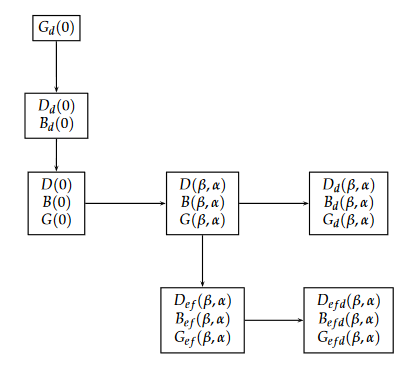
\includegraphics[scale=0.7]{32_ESFBOOK_1}
\centering
\caption{Procedimiendo de cálculo (Figura 3.3 pág 31 \cite{esf_book})}
\label{fig:fig_1}
\end{figure}

En la figura \ref{fig:fig_1} se muestra el proceso de cálculo que se debe seguir para obtener los valores de radiación efectiva incidente en el plano del generador, que después se utilizarán para calcular la energía que es capaz de entregar este.


Los pasos descritos son:
\begin{enumerate}
	\item Separar la irradiación global diaria en el plano horizontal en sus componentes de irradiación difusa y directa.
	\item Convertir la irradiación diaria a un perfil horario de irradiación global, directa y difusa en en plano horizontal.
	\item Pasar del perfil horario en el plano horizontal a un perfil con la inclinación y orientación indicada por el usuario.
	\item Aplicar las pérdidas relacionadas con el ángulo de incidencia y el nivel de suciedad.
	\item Volver a convertir el perfil horario a unos valores diarios de irradiación global, difusa y directa.
\end{enumerate}

Para poder calcular la energía producida por un generador fotovoltaico, es necesario conocer la radiación solar que incide sobre la superficie de dicho generador. Para poder predecir la energía producida por éste en un tiempo futuro, el problema que se ha de resolver es estimar la irradiancia \footnote{\textbf{Irradiancia}: densidad de potencia de radiación solar incidente en una superficie. Unidades: $\frac{W}{m^2}$} que recibirá, a partir del comportamiento de la radiación solar en ese lugar.\\

En 1960, Liu y Jordan \cite{lj60} expusieron una forma de caracterizar la radiación solar en un lugar, mediante el indice de claridad $K_T$. Éste índice es la relación entre la radiación global y la extra-terrestre, ambas en el plano horizontal. La expresión de el indice de claridad diario es:\\

\begin{equation}
\label{eqn:ktd}
K_{Td} = \frac{G_d(0)}{B_{0d}(0)}
\end{equation}
mientras que el indice de claridad mensual es la relación entre las medias mensuales de irradiación diaria:
\begin{equation}
K_{Tm} = \frac{G_{d,m}(0)}{B_{0d,m}(0)}
\end{equation}

En el código, el índice de claridad media se calcula con la siguiente expresión:
\begin{lstlisting}[style=ES6, caption={Índice de claridad diario}]
	newData.meanValues.forEach((elem, index) => {
		const Ktd = elem.meanGR / elem.B0d0
	})
\end{lstlisting}
Para cada uno de los valores medios mensuales, dividimos el valor de radiación global media entre el $B_{0d}(0)$ calculado anteriormente.

Habiendo calculado el índice de claridad, podemos utilizar su valor para calcular la Fracción de radiación difusa en el plano horizontal ($F_D=\frac{D(0)}{G(0)}$). Para ello, podemos utilizar la ecuación de Page para aproximar el dicho valor conociendo el índice de claridad.

La ecuación que define éste valor es:
\begin{equation}\label{eqn:page}
F_{Dm}=1-1,13·K_{Tm}
\end{equation}
En código, la expresión es:
\begin{lstlisting}[style=ES6, caption={Fracción de difusa}]
	newData.meanValues.forEach((elem, index) => {
		const Fd = 1 - 1.13 * elem.Ktd
	})
\end{lstlisting}
Donde elem.Ktd es el índice de claridad calculado en el paso anterior.

Al conocer, mediante la ecuación de Page el valor de la fracción de radiación difusa, podemos aplicar dicha relación para calcular los valores de radiación directa y difusa en el plano horizontal, a partir de la radiación global.
Las dos ecuaciones necesarias para calcular estos valores son:

\begin{equation}
\label{eqn:rad_difusa}
D_d(0) = F_D · G_d(0)
\end{equation}

\begin{equation}
\label{eqn:rad_directa}
B_d(0) = G_d(0) - D_d(0)
\end{equation}

En código, las expresiones toma la siguiente forma:
\begin{lstlisting}[style=ES6, caption={Radiación directa y difusa}]
	newData.meanValues.forEach((elem, index) => {
		const Dd0 = elem.Fd * elem.meanGR
		const Bd0 = elem.meanGR - Dd0
	})
\end{lstlisting}

Para cada uno de los doce valores de radiación global media, aplicamos la fracción calculada anteriormente para obtener los dos valores de radiación en el plano horizontal.

\section{Radiación en superficies inclinadas}

Para poder obtener los valores de de irradiación global en un plano inclinado a partir de valores de irradiación global en el plano horizontal se describe en la figura \ref{fig:fig_1}. El proceso de cálculo parte de los valores de irradiación global diaria en el plano horizontal, o en el caso de no tener estos valores disponibles, podemos utilizar la ecuación \ref{eqn:page} para obtener las respectivas medias mensuales de irradiación difusa y directa en el plano horizontal.
A continuación, para poder llevar a cabo las transformaciones al plano inclinado, debemos estimar los valores de irradiancia difusa, directa y global en el plano horizontal. Con estas estimaciones podemos calcular los valores correspondientes al plano inclinado.

Integrando los valores de irradiancia se obtienen las estimaciones de irradiación diaria difusa, directa y global en el plano horizontal. A estos valores les aplicaremos las pérdidas por suciedad, añadiéndole el apellido de ``efectiva`` a la irradiancia e irradiación. Será esta irradiación incidente efectiva la que se utilizará para el calculo de la energía producida por el generador.

\subsection{Estimación de irradiancia a partir de irradiación diaria}
\label{section:3.5.1}
Partiendo de los valores calculados anteriormente de irradiación diaria difusa, directa y global en el plano horizontal, podemos realizar la transformación al plano inclinado estimando el perfil de irradiancia correspondiente a cada valor de irradiación.

Como la variación solar durante una hora es relativamente baja, podemos suponer que el valor medio de irradiancia durante esa hora coincide numéricamente con irradiación horaria ($ \frac{kWh}{m^2}$).

Por otro lado, mediante análisis de series temporales se ha demostrado que la relación entre la irradiancia y la irradiación difusa es equivalente a la existente entre la irradiancia y la irradiación extra-atmosférica.
\begin{equation}
	r_D = \frac{D(0)}{D_d(0)} = \frac{B_0(0)}{B_{0d}(0)	}
\end{equation}

El factor $r_D$  se puede calcular mediante la siguiente expresión:
\begin{equation}
r_D = \frac{\pi}{T}\cdot\frac{\cos(\omega)-\cos(\omega_s)}{\omega_s\cdot\cos(\omega_s)-\sin(\omega_s)}
\end{equation}
Donde:
\begin{itemize}
\item T: Duración del día en horas
\item $\omega_s$: ángulo de amanecer, expresado en radianes
\item $\omega$: instante central de la hora correspondiente
\end{itemize}

La implementación en código es la siguiente

\begin{lstlisting}[style=ES6, caption={Cálculo de rD}]
	const rd = []
	for (let h = -12; h < 12; h++) {
			const hRad = Math.cos(deg2rad(h * 15))
			const rdval = (Math.PI / 24) * ((hRad - Math.cos(elem.ws)) / (elem.ws * 
			Math.cos(elem.ws) - Math.sin(elem.ws)))
			rd.push(rdval)
		}
\end{lstlisting}

Para cada uno de los valores horarios de -12 a 12, se calcula el angulo horario multiplicando por 15 grados y se introduce en la ecuación, obteniendo 24 valores por cada uno de los meses.

El mismo análisis muestra también la relación entre la irradiancia e irradiación global asimilable a una función dependiente de la hora solar.
\begin{equation}
r_G = \frac{G(0)}{G_d(0)} ) r_D\cdot(a+b\cdotcos(\omega))
\end{equation}
siendo:
\begin{equation}
a=0,409 - 0,5016\cdot\sin(\omega_s+\frac{\pi}{3})
\end{equation}
\begin{equation}
a=0,6609 - 0,4767\cdot\sin(\omega_s+\frac{\pi}{3})
\end{equation}

donde $\omega_s$ es negativa y está expresada en radianes.

En código, los expresiones anteriores se representan de la siguiente forma:
\begin{lstlisting}[style=ES6, caption={Cálculo de rG}]
		const rg = []
		const a = 0.409 - 0.5016 * Math.sin(elem.ws + Math.PI / 3)
		const b = 0.6609 + 0.4767 * Math.sin(elem.ws + Math.PI / 3)
		let i = 0
		for (let h = -12; h < 12; h++) {
			const hRad = Math.cos(deg2rad(h * 15))
			const rgval = rd[i] * (a + b * hRad)
			rg.push(rgval)
			i++
		}
\end{lstlisting}

\subsection{Transformación al plano del generador}
\label{section:3.5.2}

Una vez calculados los valores de irradiancia en el plano horizontal, el siguiente paso consiste en estimar los componentes de irradiancia en el plano del generador. La irradiancia directa es calculable mediante criterios geométricos, teniendo en cuenta el ángulo del cenit solar y el ángulo de incidencia en el generador.\\

Para obtener estos valores en el plano inclinado, lo primero que debemos calcular son los valores horarios de radiación global, directa y difusa en el plano horizontal, aplicando las dos relaciones, $r_D$ y $r_G$ que se han calculado en la sección anterior.

Para ello, emplearemos las siguientes ecuaciones:
\begin{equation}
D_h = r_D \cdot D_d(0)
\end{equation}
\begin{equation}
G_h = r_G \cdot G(0)
\end{equation}
\begin{equation}
B_h = G_h - D_h
\end{equation}

En código, las expresiones serían las siguientes:

\begin{lstlisting}[style=ES6, caption={Cálculo de rG}]
		const hourlyValues = []
		let hour = -12
		const dawn = rad2deg(elem.ws) / 15
		elem.dawn = dawn
		for (let i = 0; i < 24; i++) {
			const cosHour = Math.cos(deg2rad(hour * 15))
			const cosWs = Math.cos(elem.ws)
			if (cosHour > cosWs) {
				const Dh = elem.rd[i] * elem.Dd0
				const Gh = elem.rg[i] * elem.meanGR
				const Bh = Gh - Dh
				hourlyValues.push({
					Bh, Dh, Gh, cosHour, cosWs,
				})
			} else {
				hourlyValues.push({
					Bh: 0, Dh: 0, Gh: 0, cosHour, cosWs,
				})
			}
			hour++
		}
		elem.hourlyValues = hourlyValues
\end{lstlisting}

Se puede observar que para las horas en las que el coseno es menor que el coseno del ángulo de amanecer, se toman valores nulos para las radiaciones.\\

Una vez obtenidos estos valores horarios de irradiancia en el plano horizontal, el siguiente paso consiste en llevarlo al plano del generador.

El planteamiento de ésta transición es el siguiente:
\begin{itemize}
\item \textbf{Irradiancia Directa $B(\beta,\alpha)$:} ecuación basada en geometría solar (ángulo cenital) y del generador(ángulo de incidencia).
\begin{equation}
\label{eqn:B_beta_alpha}
B(\beta,\alpha) = B(0) \cdot \frac{max(0,\cos(\theta_s))}{\cos(\theta_{zs})}
\end{equation}
\item \textbf{Irradiancia Directa $D(\beta,\alpha)$:} Existen dos modelos del estado de cielo, el isotrópico y el anisotrópico. En este caso, utilizaremos el modelo anisotrópico.
\begin{equation}
D(\beta,\alpha) = D^I(\beta,\alpha)+D^C(\beta,\alpha)
\end{equation}
\begin{equation}
D^I(\beta,\alpha) = D(0)\cdot(1-k_1)\cdot\frac{1+\cos(\beta)}{2}
\end{equation}
\begin{equation}
D^C(\beta,\alpha) = D(0)\cdot k_1 \cdot \frac{max(0, \cos(\theta_s))}{\cos(\theta_{zs})}
\end{equation}
\item \textbf{Irradiancia de Albedo $R(\beta,\alpha)$:} Se considera nula por tener un porcentaje de aportación muy reducido.
\end{itemize}

Estos componentes sumados, forman la expresión de la irradiancia global en el plano del generador.
\begin{equation}
G(\beta,\alpha)=D(\beta,\alpha)+B(\beta,\alpha)+R(\beta,\alpha)
\end{equation}

En la ecuación de la irradiancia directa, uno de los elementos que influyen en el cálculo es el angulo de incidencia, cuya expresión es:
\begin{equation} \label{eqn:ang_incid}
\begin{split}
\cos(\theta_s)=sign(\phi)\cdot [ \sin(\beta)\cos(\alpha)\cos(\delta)\sin(\phi)- \\
-\sin(\beta)\cos(\alpha)\cos(\phi)\sin(\delta)]+ \\
+\sin(\beta)\sin(\alpha)\cos(\delta)\sin(\omega)+ \\
+\cos(\beta)\cos(\delta)\cos(\omega)\cos(\phi)+ \\
+\cos(\beta)\sin(\delta)\sin(\phi) \\
\end{split}
\end{equation}
Donde:
\begin{itemize}
\item \textbf{$\beta$}: Inclinación del generador
\item \textbf{$\alpha$}: Orientación del generador
\item \textbf{$\phi$}: Latitud del emplazamiento
\item \textbf{$\delta$}: Declinación
\item \textbf{$\omega$}: Hora solar
\end{itemize}
\newpage
Traducida a código, la expresión será:
\begin{lstlisting}[style=ES6, caption={Cálculo del ángulo de incidencia}]
		for (let h = -12; h < 12; h++) {
			const betaRad = deg2rad(newData.angle)
			const alphaRad = deg2rad(newData.orientation)
			const hRad = deg2rad(h * 15)
			const latRad = deg2rad(newData.latitude)
			const declRad = deg2rad(elem.decl)
			const anglIncidenciaVal =
				Math.sign(newData.latitude) *
				(Math.sin(betaRad) * Math.cos(alphaRad) * Math.cos(declRad) * 
				Math.cos(hRad) * Math.sin(latRad) -Math.sin(betaRad) * 
				Math.cos(alphaRad) *Math.cos(latRad) * Math.sin(declRad)) +
				Math.sin(betaRad) * Math.sin(alphaRad) * Math.cos(declRad) *
				Math.sin(hRad) + Math.cos(betaRad) * Math.cos(declRad) *
				 Math.cos(hRad) * Math.cos(latRad) + Math.cos(betaRad) * 
				 Math.sin(declRad) * Math.sin(latRad)
			const anglIncidencia = rad2deg(Math.acos(anglIncidenciaVal))
			const anglIncidencia = rad2deg(Math.acos(anglIncidenciaVal))
			incid.push(anglIncidencia)
			elem.incid = incid
			}
\end{lstlisting}
\newpage
Teniendo el valor del ángulo de incidencia, podemos proceder a calcular las dos componentes de irradiancia para el plano del generador.

\begin{lstlisting}[style=ES6, caption={Cálculo del ángulo de incidencia}]
newData.meanValues.forEach((elem, index) => {
		for (let i = 0; i < 24; i++) {
			const zenitRad = deg2rad(elem.zenit[i])
			const incidRad = deg2rad(elem.incid[i])
			const betaRad = deg2rad(newData.angle)
			const numerator = Math.max(0, Math.cos(incidRad))
			const denominator = Math.cos(zenitRad)
			const Btilt = elem.hourlyValues[i].Bh * (numerator / denominator)
			const k1 = elem.hourlyValues[i].Bh / elem.B00[i]
			const DcTilt = elem.hourlyValues[i].Dh * k1 * (numerator / denominator)
			const DiTilt = elem.hourlyValues[i].Dh * (1 - k1) * ((1 + Math.cos(betaRad)) / 2)
			const Dtilt = DcTilt + DiTilt
			const Gtilt = Btilt + Dtilt
			elem.hourlyValues[i] = {
				...elem.hourlyValues[i],
				Btilt,Dtilt,DcTilt,DiTilt,Gtilt,cosZenit: Math.cos(zenitRad),
			}
		}
	})
\end{lstlisting}

Con estos cálculos obtenemos la irradiancia global incidente, es decir, en el plano del generador. El siguiente es añadirle el apellido de ``efectica'' aplicándole las pérdidas por ángulo de incidencia y suciedad.

\subsection{Pérdidas por ángulo de incidencia y suciedad}
\label{section:3.5.3}

Al tratarse de sistemas estáticos, la radiación incidente en un módulo fotovoltaico está frecuentemente desviada de la normal a la superficie del módulo. Esta desviación, cuantificada por el ángulo de incidencia [eq. \ref{eqn:ang_incid}], es causa de pérdidas por reflexión.

Por otro lado, la suciedad acumulada en la superficie del módulo altera las propiedades angulares del mismo y reduce la capacidad de transmisión del vidrio.

Estos dos fenómenos reducen la irradiancia que es aprovechada por el módulo. Para el caso de la radiación directa, la expresión de irradiancia efectiva es la siguiente:
\begin{equation}
B_{ef}(\beta, \alpha)= B(\beta,\alpha)\cdot\frac{T_{sucio}(0)}{T_{limpio}(0)}\cdot(1-FT_B(\theta_s))
\end{equation}
donde $FT_B(\theta_s)$ es el factor de pérdidas angulares para la irradiancia directa, calculable mediante la ecuación:
\begin{equation}
FT_B(\theta_s) = \frac{exp(-\frac{\cos(\theta_s)}{a_r})-exp(-\frac{1}{a_r})}{1-exp(-\frac{1}{a_r})}
\end{equation}

Los valores del coeficiente de pérdidas angulares deben ser determinados de forma experimental. En la tabla quedan recogidos algunos valores característicos de un módulo de silicio monocristalino convencional para los diferentes grados de suciedad. Además en la tabla también se recogen los valores de la transmitancia al interior del módulo en incidencia normal respecto a uno limpio $\frac{T_{sucio}(0)}{T_{limpio}(0)}$.

\begin{table}[ht]
\centering
\begin{tabular}{llll}
\hline
Grado de suciedad & $\frac{T_{sucio}(0)}{T_{limpio}(0)}$ & $a_r$ & $c_2$ \\
Limpio            & 1                                                          & 0,17 & -0.069 \\
Bajo              & 0,98                                                       & 0,20 & -0.054 \\
Medio             & 0,97                                                       & 0,21 & -0.049 \\
Alto              & 0,92                                                       & 0,22 & -0.023
\end{tabular}
\label{tab:perdidas_suciedad}
\caption{Coeficiente de pérdidas angulares y transmitancia relativa en incidencia normal para diferentes niveles de suciedad }
\end{table}
El cálculo del coeficiente $FT_B(\theta_s)$, en código, toma este aspecto:
\begin{lstlisting}[style=ES6, caption={Cálculo del coeficiente $FT_B(\theta_s)$}]
newData.TDirtTClean = TDirtTClean
newData.ar = ar
newData.c1 = c1
newData.c2 = c2
const FTB = (Math.exp(-Math.cos(tiltRad) / ar) - 
Math.exp(-1 / ar)) / (1 - Math.exp(-1 / ar))
\end{lstlisting}


Para la componente de isotrópica existe otra expresión que depende del ángulo de inclinación del generador, del coeficiente de pérdidas angulares y de dos coeficientes de ajuste $c_1$ y $c_2$. El primero de ellos toma un valor constante $c_1=\frac{4}{3\pi}$. El segundo depende linealmente de $a_r$ según se recoge en la tabla. En ésta expresión el ángulo $\beta$ está en radianes.
\begin{equation}
FT_D \simeq exp[-\frac{1}{a_r}\cdot(c_1\cdot(\sin\beta + \frac{\pi-\beta-\sin\beta}{1+\cos\beta	})+c_2\cdot(\sin\beta + \frac{\pi-\beta-sin\beta}{1+\cos\beta})^2)]
\end{equation}
\newpage
Para estas componentes el cálculo de irradiancia efectiva es similar al de la irradiancia directa. Para la componente difusa circunsolar emplearemos el factor de pérdidas angulares de la irradiancia efectiva:

\begin{equation}
D_{ef}^I(\beta, alpha) = D^I(\beta, alpha) \cdot \frac{T_{sucio}(0)}{T_{limpio}(0)} \cdot (1-FT_D(\beta))
\end{equation}

\begin{equation}
D_{ef}^C(\beta, alpha) = D^C(\beta, alpha) \cdot \frac{T_{sucio}(0)}{T_{limpio}(0)} \cdot (1-FT_B(\beta))
\end{equation}

En código las ecuaciones toman esta forma:
\begin{lstlisting}[style=ES6, caption={Cálculo de las componentes efectivas}]
				const expFTD =
					-(1 / ar) *
					(c1 * (Math.sin(betaRad) + (Math.PI - betaRad - Math.sin(betaRad)) / (1 + 
					Math.cos(betaRad))) +
						c2 * Math.pow(Math.sin(betaRad) + (Math.PI - betaRad - 
						Math.sin(betaRad)) / (1 + Math.cos(betaRad)), 2))
				const FTD = Math.exp(expFTD)

				const Btilt = elem.hourlyValues[i].Btilt * TDirtTClean * (1 - FTB)
				const DiTilt = elem.hourlyValues[i].DiTilt * TDirtTClean * (1 - FTD)
				const DcTilt = elem.hourlyValues[i].DcTilt * TDirtTClean * (1 - FTB)
\end{lstlisting}

Antes de pasar a calcular la energía producida por el generador configurado, se va a llevar a cabo una filtración de datos para eliminar los valores horarios entre el atardecer y el amanecer.
Para ello, aplicamos este algoritmo a los datos calculados anteriormente
\begin{lstlisting}[style=ES6, caption={Selección de los valores clave}]
	newData.meanValues.forEach((elem, index) => {
		const significantValues = []
		elem.hourlyValues.forEach((value, index) => {
			if (Math.abs(value.hour) < Math.abs(elem.dawn)) {
				significantValues.push(value)
			}
		})
		elem.significantValues = significantValues
	})
\end{lstlisting}
Como se observa, los valores horarios menores al amanecer, en valor absoluto, no se introducen en la lista de valores significativos.

\section{Cálculo de la energía producida por el generador}

Una vez calculados los valores de radiación en el plano del generador, el siguiente paso será proceder a estimar la energía que es capaz de producir dicho generador conectado a red.\\

En el caso de la aplicación desarrollada en el proyecto, el objetivo es estimar la energía máxima que será capaz de producir un sistema fotovoltaico conectado a red.

\subsection{Definición de un SFCR}

Un Sistema Fotovoltaico Conectado a Red (SFCR) es un sistema cuya función es producir energía eléctrica en una condiciones específicas, de tal manera que ésta pueda ser inyectada en la red eléctrica convencional. Para ello, un SFCR se compone del propio generador fotovoltaico, un inversor DC/AC y un conjunto de protecciones eléctricas. Tal y como se muestra en la figura \ref{fig:sfcr}.

\begin{figure}[ht]
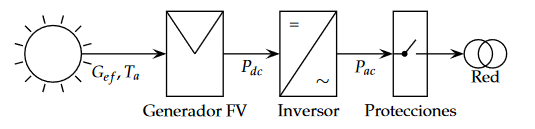
\includegraphics[scale=0.7]{SFCR}
\centering
\caption{Esquema de un SFCR (Figura 6.1 pág 65 \cite{esf_book})}
\label{fig:sfcr}
\end{figure}

La energía producida por un SFCR es consumida total o parcialmente en el emplazamiento de la instalación, o en sus cercanías. La energía sobrante es inyectada a la red de distribución, y a cambio el propietario es compensado económicamente a través de sistemas de retribución tales como: la retribución con prima o el balance neto.

A diferencia de un sistema autónomo o de bombeo, el diseño de SFCR no necesita considerar un consumo mínimo a satisfacer. Con este mecanismo, el objetivo es que la producción anual del sistema sea la máxima posible sin tomar en consideración los consumos cercanos.

\subsection{Configuración de los elementos del sistema}

A la hora de estimar la energía producida por un SFCR, debemos definir las características nominales de los componentes que forman parte de este, como se muestra en la figura \ref{fig:sfcr}.
Con el objetivo de reducir al máximo la complejidad de la aplicación de cara al usuario final (cuyos conocimientos de fotovoltaica, de media, serán reducidos) se han fijado unos valores standard para el módulo fotovoltaico, la configuración del generador y el inversor.

\newpage

Estos valores se muestran en las siguientes tablas:
\begin{itemize}
\item \textbf{Configuración del módulo} El módulo elegido es uno disponible comercialmente, fabricado por JINKO SOLAR, modelo JKM320PP \footnote{\textit{Módulos solar JINKO SOLAR, modelo JKM320PP \url{https://autosolar.es/pdf/Ficha-Tecnica-Jinko-Solar-305-320W.pdf}}}

\begin{table}[ht]
\centering
\begin{tabular}{llll}
\hline
G*               & 1000 $ \frac{W}{m^2}$    \\
V_{oc}*          & 46,4 V                   \\
I_{sc}*          & 9,05 A                   \\
V_{mpp}*         & 37,4 V                   \\
I_{mpp}*         & 8,56 A                   \\
N_{cs}           & 12                       \\
N_{cp}           & 6                        \\
TONC             & 45 $\degree$             \\
T_c              & 25 $\degree$             \\
V_t              & 0,025V	                \\
m                & 1,3                      \\
Área modulo      & $1,957 \times 0,992 m^2$ \\
Potencia Nominal & 320 Wp                   \\  
\end{tabular}
\label{tab:module_conf}
\caption{Configuración módulo standard }
\end{table}
\item \textbf{Inversor}:
\begin{table}[ht]
\centering
\begin{tabular}{llll}
\hline
k_0      & 0,01  \\
k_1      & 0,025 \\
k_2      & 0,05  \\
Potencia & 40 kW \\
V_{min}  & 420 V \\
V_{max}  & 750 
\end{tabular}
\label{tab:inverter_conf}
\caption{Configuración del inversor }
\end{table}

\item \textbf{Generador} La configuración del generador será de \textbf{12} módulos en serie y \textbf{11} módulos en paralelo.

\end{itemize}


\subsection{Funcionamiento de una célula solar}

Para poder llevar a cabo la estimación de la energía producida por el generador, debemos conocer como influye factores como la radiación o la temperatura en una célula solar y en los valores de tensión y corriente que se alcanzan en dichas condiciones.

Existen dos puntos clave que definen una célula solar, la corriente de cortocircuito ($I_{sc}$) y la tensión de circuito abierto ($V_{oc}$). 
Estos dos parámetros suelen estar disponibles en la información asociada a una célula y se pueden relacionar mediante la siguiente ecuación:

\begin{equation}
I = I_{sc} \cdot \left[ 1 - exp\left(\frac{e\cdot(V_{oc}-V}{m \cdot k \cdot T_c}\right)\right]
\end{equation}

\subsubsection{Punto de máxima potencia}

Superpuesta a la curva de corriente-tensión, la figura \ref{fig:mpp} incluye la relación entre la potencia y la tension. Como se puede observar, existe un punto donde dicha potencia es máxima, antes de volver a experimentar una bajada. Las coordenadas de dicho punto vienen definidas por la condición $\frac{dP}{dV} = 0$. En dicho punto, la potencia entregada por la célula es máxima y será considerada como potencia nominal: $P_{mpp} = V_{mpp} \cdot I_{mpp}$. La unidades de dicha potencia son los vatios pico (Wp), indicando así que se trata de la máxima potencia alcanzable.\\

\begin{figure}[ht]
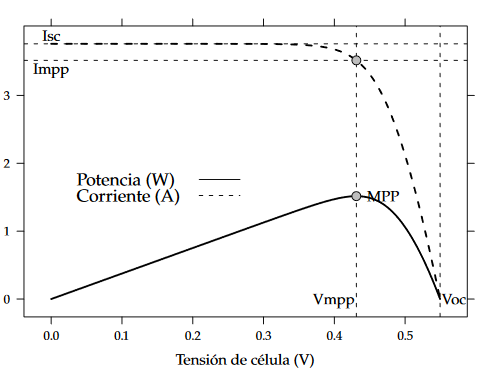
\includegraphics[scale=0.7]{MPP}
\centering
\caption{Curvas corriente-tensión (línea discontinua) y potencia-tensión (línea contínua) de una célula solar ( $T_a=20\degree C$ y $G=800 \frac{W}{m^2}$) (Figura 4.6 pág 49) \cite{esf_book})}
\label{fig:mpp}
\end{figure}


Como la célula funciona en corriente continua, su potencia es $ P = V \cdot I $ y por tanto:

\begin{equation}
\begin{align}
\frac{d(I \cdot V)}{dV} &= V \cdot \frac {dI}{dV}+I\cdot\frac{dV}{dV}\\
dP &= V\cdotdI+I\cdotDV
\end{align}
\end{equation}

En el punto de máxima potencia se cumplirá:
\begin{equation}
\frac{dI}{dV}=-\frac{I_{mpp}}{V_{mpp}}
\end{equation}
\subsubsection{Factor de forma y eficiencia}

Como se puede observar en la figura \ref{fig:mpp}, el área encerrada por el rectángulo $I_{mpp}\cdot V_{mpp}$ es inferior al definido por $I_{sc} \cdot V_{oc}$. La relación entre estas dos áreas, se conoce como factor de forma, y toma la siguiente expresión:
\begin{equation}
\label{eqn:FF}
FF = \frac{I_{mpp} \cdot V_{mpp}}{I_{sc} \cdot V_{oc}}
\end{equation}

Este factor toma valores entre 0,7 y 0,8 variando poco de unas células a otras. Conociendo los valores de $I_{sc}$ y $V_{oc}$ es posible calcular la potencia en el punto de máxima potencia, dado que $P_{mpp}=FF \cdot I_{sc} \cdot V_{oc}$.

Por otra parte, la calidad de una célula se puede cuantificar según la ecuación de la eficiencia de conversión:
\begin{equation}
\eta = \frac{I_{mpp} \cdot V_{mpp}}{P_L}
\end{equation}
donde $P_L$ representa la potencia luminosa que incide en la célula.

\subsubsection{Influencia de la temperatura y la radiación}

Es importante tener en cuenta, a la hora de entender el funcionamiento de una célula solar, la influencia de los dos principales factores externos: la temperatura ambiente y la iluminación incidente o radiación.

El aumento de la temperatura tiene una influencia notable en la tensión de circuito abierto de la célula según el valor $dV_{oc}/dT_c$. donde $T_c$ es la temperatura de la célula, dependiente de la temperatura ambiente y la radiación incidente. La forma de calcular ésta temperatura depende de las características constructivas del módulo que encapsula a la célula. Si el fabricante no nos ofrece información sobre este valor, para células de silicio cristalino se común tomar el siguiente valor:
\begin{equation}
\frac{dV_{oc}}{dT_c}=-2,3\frac{mV}{ \circ C}
\end{equation}

\subsubsection{Cálculo del punto de máxima potencia}

Anteriormente, se ha mostrado la relación entre la temperatura y la irrandiancia con la tension de \textit{circuito abierto} $V_{oc}$ y la corriente de \textit{cortocircuito} $I_{sc}$. Además, los fabricantes suelen incluir estos dos valores en el punto de máxima potencia en las condiciones estándar de medida.

Por tanto, para poder estimar el comportamiento de la célula en otras condiciones, es necesario trasladar estos parámetros a los valores de temperatura e irradiancia en dicha situación.\\

El procedimiento de cálculo consistirá en comenzar asumiendo que el factor de forma es constante, para calcular los valores de $I_{sc}$ y $V_{oc}$ en las condiciones de temperatura y radiación del emplazamiento. Posteriormente realizaremos los cálculos para tomar en cuenta la variación del factor de forma.



\subsection{Asociación de dispositivos fotovoltaicos}

Por defecto, las características eléctricas de una sola célula no son suficientes para alimentar una carga convencional. Por lo tanto, es necesario realizar agrupaciones en serie y en paralelo de varias de estas células en lo que conocemos como módulo fotovoltaico para entregar de esta manera los valores de tensión y corriente adecuados para la carga.

Además, un módulo fotovoltaico protege físicamente de la intemperie y aísla eléctricamente al conjunto de células, otorgando la rigidez mecánica necesaria.

\subsubsection{Modelado de un módulo}

Conociendo el comportamiento de una célula solar independiente, podemos trasladarlo al módulo teniendo en cuenta la configuración de éste, sobre todo el numero de células en serie y en paralelo que lo componen.

Para modelar el funcionamiento de un módulo podemos realizar las siguientes suposiciones:
\begin{itemize}
\item Los efectos de la resistencia en paralelo son despreciables.
\item La resistencia serie es independiente de las condiciones de operación.
\item La corriente fotogenerada ($I_L$) es igual a la corriente de cortocircuito.
\item En cualquier condición de operación: $exp(\frac{V+I\cdotR_s}{V_t}) > 1$
\end{itemize}

En un módulo compuesto por $N_{cs}$ células en serie y $N_{cp}$ ramas en paralelo, y suponiendo que todas las células del módulo tienes características idénticas, la tensión de dicho módulo es $V_m= N_{cs} \cdot V_c$ y la corriente del módulo es $I_m = N_{cp} \cdot I_c$ siendo $I_c$ y $V_c$ la corriente y la tensión de  una célula, respectivamente.

Dadas estas suposiciones, la curva de la corriente de módulo toma la siguiente expresión:

\begin{equation}
I_m = I_{sc} \cdot \left( 1 - exp \left(\frac{V_m - V_{oc} + I_m \cdot R_s}{Vt}\right) \right)
\end{equation}

Supondremos que la corriente de cortocircuito depende exclusivamente y de forma linea de la irradiancia:
\begin{equation}
\label{eqn:I_sc}
I_sc = G_{ef} \cdot \frac{I_{sc}^*}{G_{stc}}
\end{equation}
y la tensión de circuito abierto depende exclusivamente de la temperatura de célula, y decrece linealmente con ella:
\begin{equation}
\label{eqn:V_oc}
V_{oc}(T_c) = V_{oc}^* + (T_c - T_c^*) \cdot \frac{dV_{oc}}{dT_c}
\end{equation}

Como ya hemos mencionado anteriormente, si no hay información específica del por parte del fabricante, para módulos de silicio cristalino es habitual emplear el valor:
\begin{equation}
\frac{dV_{oc}}{dT_c}=-2,3\frac{mV}{ celula \degree C}
\end{equation}

\subsubsection{Comportamiento térmico del módulo}
\label{section:term_behaviour}

En las ecuaciones anteriores se hace referencia a las condiciones estándar de medida. En estas condiciones, la temperatura de la célula es de $25\degree C$. Sin embargo, la temperatura de operación de la célula es diferente y depende del balance de potencias del módulo.

El módulo recibe potencia luminosa, absorbiendo la fracción de ésta que no se refleja al exterior. De dicha fracción parte es transformada en energía eléctrica mientras que el resto se entrega en forma de calor al entorno.

Para simplificar podemos asumir que el incremento de la temperatura de la célula respecto a la ambiente depende linealmente de la irradiancia incidente en ésta. El coeficiente de proporcionalidad depende de muchos factores, tales como el modo de instalación del módulo, la velocidad del viento, la humedad del ambiente o las características constructivas del laminado que cubre las células.

Todos estos factores quedan recogidos en un valor único representado por la temperatura de operación nominal de la célula (NOCT o TONC), definida como aquella que alcanza una célula cuando su módulo trabaja en las siguientes condiciones:
\begin{itemize}
\item Irradiancia: $G=800 \frac{W}{m^2}$.
\item Espectro: el correspondiente $AM=1,5$.
\item Incidencia normal.
\item Temperatura ambiente: $T_a = 20 \degree C$.
\item Velocidad del viento:  $ v_v = 1 \frac{m}{s}$.
\end{itemize}

\begin{equation}
\label{eqn:T_c}
T_c = T_a + \frac{G_{ef}\cdot(TONC - 20)}{800}
\end{equation}

Como se puede observar, en la temperatura de la célula influyen tanto la temperatura ambiente como la radiación global eficaz. Al trabajar con valores horarios, es necesario conocer el valor de la temperatura ambiente en cada hora del día.



El procedimiento para calcular los valores de temperatura ambiente horarios para cada uno de los meses en el emplazamiento indicado por el usuario no es trivial pues normalmente no suele haber un registro histórico de temperaturas. Para ello vamos a utilizar el proceso descrito en el documento \cite{temp_paper}.

En dicho documento se describe un proceso para desarrollar un perfil horario de temperaturas partiendo de una temperatura máxima y mínima.

Los pasos a seguir son:

\begin{enumerate}
\item \textbf{Obtención de la temperatura mínima y máxima}: Lo primero que necesitamos para poder realizar el perfil de temperatura es conocer los valores de temperatura mínima y máxima para cada uno de los meses. Para ello utilizaremos la API que nos proporciona AEMET a través de su plataforma de OPENDATA \footnote{\textit{AEMET OPENDATA}: Base de datos abierta de información climatológica, entre otras \url{https://opendata.aemet.es}}. Para ello buscamos en su base de datos la estación climatológica más cercana a las coordenadas del usuario y solicitamos la información necesaria, en este caso las temperaturas mensuales de un año entero.
\item \textbf{Cálculo del ángulo de amanecer}: Una vez obtenidos los valores de temperatura mensuales, el siguiente paso es calcular el ángulo de amanecer para cada uno de los 12 días normales, como se ha hecho en pasos anteriores mediante la declinación. Para ello empleamos las dos ecuaciones:
\begin{equation}
\delta = 23.45 \cdot \sin\left(\frac{2\pi \cdot (d_N + 284) }{365}\right)
\end{equation}
\begin{equation}
\begin{align}
\cos(\omega_s) &= -\tan(\delta) \cdot \tan(lat)\\
\omega_s &= acos(\omega_s)
\end{align}
\end{equation}
donde:
\begin{itemize}
\item $d_N$: Día normal correspondiente \ref{tab:dias_promedio}
\item lat: Latitud del emplazamiento
\end{itemize}
\item \textbf{Calcular los valores de $T_m$ y $T_r$ }: En el documento mencionado, el primer paso para llegar al perfil de temperaturas, una vez obtenidos los valores de $T_{max}$ y $T_{min}$ es calcular los dos valores intermedios:
\begin{equation}
T_m = \frac{T_{max} + T_{min} }{2}
\end{equation}

\begin{equation}
T_r = \frac{T_{max} - T_{min} }{2}
\end{equation}

\item \textbf{Calcular la matriz de $T_a$}: Una vez obtenidos los dos valores intermedios de $T_m$ y $T_r$, el siguiente paso es calcular la matriz de valores de temperatura ambiental $T_a$ para cada hora. Para ello el documento nos indica que debemos calcular tres valores que denomina $a_1$, $a_2$, $a_3$. Utilizaremos estos tres valores para calcular $T_1$,$T_2$,$T_3$, eligiendo uno u otro en función del angulo solar. Las expresiones de estos tres valores se indican a continuación:
\begin{equation}
a_1 = \frac{12\pi \cdot (\omega_s - \omega)}{21 \pi + 12 \cdot \omega_s}
\end{equation}
\begin{equation}
a_2 = \frac{\pi \cdot (3\pi - 12\omega)}{3\pi - 12\omega}
\end{equation}
\begin{equation}
a_3 = \frac{\pi \cdot (24\pi +  12 \cdot (\omega_s - \omega) }{21 \cdot \pi + 12 \cdot \omega_s}
\end{equation}
donde $\omega$ es el ángulo solar y $\omega_s$ es el ángulo amanecer.

Con estos tres valores podemos calcular la otra terna de $T_1$,$T_2$ y $T_3$ con las siguientes ecuaciones:
\begin{equation}
T_1 = T_m - Tr \cdot cos(a_1)
\end{equation}
\begin{equation}
T_2 = T_m + Tr \cdot cos(a_2)
\end{equation}
\begin{equation}
T_3 = T_m - Tr \cdot cos(a_3)
\end{equation}

\item \textbf{Selección del valor clave}: en la matriz de temperatura ambiente introduciremos uno de los tres valores en función de si el ángulo solar es menor al del amanecer, si está entre en amanecer y $\frac{\pi}{4}$ o si es menor que $\frac{\pi}{4}$.

\end{enumerate}
\newpage
En código, todo este proceso toma la siguiente forma:
\begin{lstlisting}[style=ES6, caption={Cálculo de la temperatura ambiente}]
	const wp = Math.PI / 4;
	const Tm = (Tmax + Tmin) / 2;
	const Tr = (Tmax - Tmin) / 2;
	const Ta = [];
	const decl = 23.45 * Math.sin((2 * Math.PI * (normalDays[index] + 284)) / 365);
	const cosWs = -Math.tan(deg2rad(decl)) * Math.tan(deg2rad(latitude));
	const ws = -Math.acos(cosWs);
	for (let h = -12; h < 12; h++) {
		const w = Math.cos(deg2rad(h * 15));
		const a1 = (Math.PI * 12 * (ws - w)) / (21 * Math.PI + 12 * ws);
		const a2 = (Math.PI * (3 * Math.PI - 12 * w)) / (3 * Math.PI - 12 * ws);
		const a3 = (Math.PI * (24 * Math.PI + 12 * (ws - w))) / (21 * Math.PI + 12 * ws);
		const T1 = Tm - Tr * Math.cos(a1);
		const T2 = Tm + Tr * Math.cos(a2);
		const T3 = Tm - Tr * Math.cos(a3);
		if (w <= ws) {
			Ta.push(T1);
		} else if (w > ws && w <= wp) {
			Ta.push(T2);
		} else if (w > wp) {
			Ta.push(T3);
		}
	}
\end{lstlisting}

Habiendo obtenido la matriz de temperatura ambiente, el siguiente paso es utilizar estos valores para calcular la temperatura de la célula $T_c$ con la ecuación \ref{eqn:T_c} necesaria para calcular la tensión de circuito abierto $V_{oc}$.
\newpage
En código sería:
\begin{lstlisting}[style=ES6, caption={Cálculo de la temperatura de célula}]
	const cellTempProfiles = tempProfiles.map(({ hourlyTa, Tmax, Tmin }, indexA) => {
		const meanValue = radiationData.meanValues[indexA];
		const TCProfile = hourlyTa.map((temp, indexB) => {
			const Gef = meanValue.hourlyValues[indexB].Gtilt * 1000;
			const Tc = temp + (Gef * (moduleData.TONC - 20)) / 800; 
			return Tc;
		});
		return { TCProfile, month: index + 1, Tmax, Tmin };
	});
\end{lstlisting}

Como se observa en el código, para cada uno de los valores horarios utilizamos la $G_{ef}$ en el plano inclinado (en el código aparece como \textit{Gtilt}) y la temperatura ambiente calculada anteriormente ( en el código es \textit{temp} ) para calcular la $T_c$.

Conociendo ya los valores horarios de temperatura de la célula, procedemos a calcular la tensión de circuito abierto $V_{oc}$ utilizando la expresión \ref{eqn:V_oc_cs} que, como se puede observar es la misma que \ref{eqn:V_oc} pero añadiendo el número de células en serie para convertirlo a tensión del módulo
\begin{equation}
\label{eqn:V_oc_cs}
V_{oc}(T_c) = V_{oc}^* + (T_c - T_c^*) \cdot \frac{dV_{oc}}{dT_c} \cdot N_{cs}
\end{equation}
que en código quedaría de la siguiente forma:
\begin{lstlisting}[style=ES6, caption={Cálculo de la tensión de circuito abierto}]
	const VocProfile = cellTempProfile.map(({ TCProfile }, index) => {
		const VocArray = TCProfile.map((temp) => {
			const Voc = moduleData.VocStar + (temp - moduleData.Tc) 
			* (-2.3 / 1000) * moduleData.Ncs;
			return Voc;
		});
		5return VocArray;
	});

\end{lstlisting}
\newpage
Por último, podemos calcular el valor de la corriente de cortocircuito $I_{sc}$ que depende linealmente del valor de irradiancia según se indica en la expresión \ref{eqn:I_sc} que en código resulta de la siguiente forma:

\begin{lstlisting}[style=ES6, caption={Cálculo de la corriente de cortocircuito}]
	const IscProfile = radiationData.meanValues.map(({ hourlyValues }) => {
		const IscArray = hourlyValues.map(({ Gtilt }) => {
			const IscValue = Gtilt * 1000 * (moduleData.IscStar / moduleData.Gstar);
			return IscValue;
		});
		return IscArray;
	});
\end{lstlisting}

\subsubsection{Factor de forma variable}

Los cálculos anteriores se han realizado suponiendo que el factor de forma $FF$ es constante, por tanto, de la expresión \ref{eqn:FF}, si suponemos que FF es constante, se podrían extraer los valores de tensión y corriente en el punto de máxima potencia ya que si
\begin{equation}
FF = FF^*
\end{equation}
entonces
\begin{equation}
\frac{I_{mpp} \cdot V_{vmpp}}{I_{sc} \cdot V_{oc}} = \frac{I_{mpp^*} \cdot V_{vmpp}^*}{I_{sc}^* \cdot V_{oc}^*}
\end{equation}

pudiendo así obtener los valores de $I_{mpp}$ y $V_{vmpp}$.

Estos cálculos se realizaron como una primera aproximación que sirvió para comprobar si el proceso de cálculo de la radiación eficaz incidente eran correcto.

Sin embargo, hacer esta suposición nos aleja en cierta manera de ofrecer una estimación los más próxima a la realidad posible.

Por tanto, para intentar aproximarnos los máximo posible a una estimación acertada, eliminaremos dicha suposición y tendremos en cuenta la variación del factor de forma. Para ello, utilizaremos el siguiente proceso:
\begin{enumerate}
\item \textbf{Cálculo de la tensión térmica, $V_t$, a temperatura de la célula}: Calcularemos el valor de $V_{t}$ a 25 $\degree$ C con la expresión:
\begin{equation}
V_{tn} = \frac{V_t \cdot (273 + 25)}{300}
\end{equation} 
\begin{lstlisting}[style=ES6, caption={Cálculo de $V_{tn}$}]
const Vtn = (moduleData.Vt * (273 + 25)) / 300;
\end{lstlisting}
\item \textbf{Cálculo de $R_s^*$}: El segundo paso consiste en calcular el valor de resistencia en serie con los valores STC:
\begin{equation}
R_s^* = \frac{\frac{V_{oc}^*}{N_{cs}} - \frac{V_{mpp}^*}{N_{cs}} + m \cdot V_{tn} \cdot \ln \left( 1 - \frac{I_{mpp}^*}{I_{sc}^*}\right)}{\frac{I_{mpp}^*}{N_{cp}}}
\end{equation}
En código quedaría:
\begin{lstlisting}[style=ES6, caption={Cálculo de $R_s^*$}]
	const RsStar =
		(moduleData.VocStar / moduleData.Ncs -
			moduleData.VmppStar / moduleData.Ncs +
			moduleData.m * Vtn * Math.log(1 - moduleData.ImppStar / moduleData.IscStar)) /
		(moduleData.ImppStar / moduleData.Ncp);
\end{lstlisting} 
\item \textbf{Cálculo de $r_s$}: Utilizando el valor $R_s^*$ calculado en el paso anterior junto con los valores de $V_{oc}$ y $I_{sc}$ calculados anteriormente podemos calcular $r_s$ que se utilizará más adelante en proceso. La ecuación que lo define viene dada por
\begin{equation}
r_s = R_s^* \cdot \left( \frac{N_{cs}}{N_{cp}} \cdot \frac{I_{sc}}{V_{oc}}}\right)
\end{equation}
y el equivalente en código es
\begin{lstlisting}[style=ES6, caption={Cálculo de $r_s$}]
	const rs = VocProfile.map((VocArray, arrIndex) => {
		return VocArray.map((VocValue, valIndex) => {
			return RsStar * ((moduleData.Ncs / moduleData.Ncp) 
			* (IscProfile[arrIndex][valIndex] / VocValue));
		});
	});
\end{lstlisting} 

Como se puede observar en la línea 4 del código, el valor de $I_{sc}$ viene acompañado por dos índices entre corchete, esto es porque en todo momento estamos trabajando con valores horarios de cada día promedio correspondiente a cada uno de los 12 meses del año, por tanto, estamos trabajando una una matriz de 12x24, de ahí el uso de los dos índices. 

\item \textbf{Cálculo de $k_{oc}$}: A continuación, utilizando los valores de temperatura ambiente obtenidos con anterioridad junto con la tensión de circuito abierto, calcularemos $k_{oc}$ mediante la expresión:
\begin{equation}
k_{oc} = \frac{V_{oc} / N_{cs}}{m \cdot V_t \cdot \frac{T_c + 273}{300}}
\end{equation}
En código tendría este forma:
\begin{lstlisting}[style=ES6, caption={Cálculo de $k_{oc}$}]
	const koc = VocProfile.map((VocArray, arrIndex) => {
		return VocArray.map((VocValue, valIndex) => {
			return VocValue / moduleData.Ncs / (moduleData.m * ((moduleData.Vt *
			(cellTempProfile[arrIndex].TCProfile[valIndex] + 273)) / 300));
		});
	});
\end{lstlisting} 
\end{enumerate}

Con éstos cálculos previos, éste método propone localizar el punto de máxima potenica de forma aproximada mediante las ecuaciones:
\begin{equation}
i_{mpp} = 1 - \frac{D_M}{k_{oc}}
\end{equation}
\begin{equation}
v_{mpp} = 1 - \frac{\ln(k_{oc}/D_M)}{k_{oc}}-r_s\cdot i_{mpp}
\end{equation}

donde:
\begin{equation}
D_M = D_{M0} + 2 \cdot r_s \cdot D_{M0}^2
\end{equation}

\begin{equation}
D_{M0} = \frac{k_{oc}-1}{k_{oc} - \ln k_{oc}}
\end{equation}

En código el proceso a seguir para llegar a los dos valores de $i_{mpp}$ y $v_{mpp}$ es el siguiente:

\begin{lstlisting}[style=ES6, caption={Cálculo de $D_{M0}$}]
	const DM0 = koc.map((kocArray, arrIndex) => {
		return kocArray.map((kocValue, valIndex) => {
			return (kocValue - 1) / (kocValue - Math.log(kocValue));
		});
	});
\end{lstlisting} 

\begin{lstlisting}[style=ES6, caption={Cálculo de $D_{M}$}]
	const DM = DM0.map((DM0Array, arrIndex) => {
		return DM0Array.map((DM0Value, valIndex) => {
			return DM0Value + 2 * rs[arrIndex][valIndex] * Math.pow(DM0Value, 2);
		});
	});
\end{lstlisting} 

\begin{lstlisting}[style=ES6, caption={Cálculo de $i_{mpp}$}]
	const impp = DM.map((DMArray, arrIndex) => {
		return DMArray.map((DMValue, valIndex) => {
			return 1 - DMValue / koc[arrIndex][valIndex];
		});
	});
\end{lstlisting} 

\begin{lstlisting}[style=ES6, caption={Cálculo de $v_{mpp}$}]
	const vmpp = impp.map((imppArray, arrIndex) => {
		return imppArray.map((imppValue, valIndex) => {
			return 1 - Math.log(koc[arrIndex][valIndex] / 
			DM[arrIndex][valIndex]) / koc[arrIndex][valIndex] - 
			rs[arrIndex][valIndex] * imppValue;
		});
	});
\end{lstlisting} 

Por último, multiplicando los valores de $i_{mpp}$ y $v_{mpp}$ por $I_{sc}$ y $V_{oc}$ respectivamente, obtendremos los valores de $I_{mpp}$ y $V_{mpp}$ que serán los que utilizaremos para calcular la potencia entregada por el generador en el punto de máxima potencia.

\begin{lstlisting}[style=ES6, caption={Cálculo de $V_{mpp}$ y $I_{mpp}$}]
	const Vmpp = vmpp.map((vmppArray, arrIndex) => {
		return vmppArray.map((vmppValue, valIndex) => {
			return vmppValue * VocProfile[arrIndex][valIndex];
		});
	});
	const Impp = impp.map((imppArray, arrIndex) => {
		return imppArray.map((imppValue, valIndex) => {
			return imppValue * IscProfile[arrIndex][valIndex];
		});
	});

\end{lstlisting} 

Una vez calculados los valores de $I_{mpp}$ y $V_{mpp}$ podemos pasar a obtener los valores horarios de la potencia en el MPP, simplemente multiplicando los valores de corriente y tensión: $P_{mpp} = I_{mpp} \cdot V_{mpp}$.
\newpage

\begin{lstlisting}[style=ES6, caption={Cálculo de $P_{mpp}$}]
	const calculatePmpp = (ImppProfile, VmppProfile) => {
		const PmppProfile = ImppProfile.map((ImppArray, dayIndex) => {
			const PmppArray = ImppArray.map((ImppValue, hourIndex) => {
				return ImppValue * VmppProfile[dayIndex][hourIndex];
			});
			return PmppArray;
		});
		return PmppProfile;
	};

\end{lstlisting} 

\subsubsection{Cálculo final de potencias y energías}

La potencia que obtenemos es la de un solo módulo. Para conocer la potencia que va a ser capaz de entregar el generador, debemos tener en cuenta su configuración de módulos en serie y en paralelo, y multiplicar estos valores de la siguiente manera:

\begin{lstlisting}[style=ES6, caption={Cálculo de la potencia del generador}]
	const calculateGeneratorPower = (PmppProfile) => {
		const PdcProfile = PmppProfile.map((PmppArray) => {
			return PmppArray.map((PmppValue) => {
				return PmppValue * generatordata.seriesModules * generatordata.parallelModules;
			});
		});
		return PdcProfile;
	};

\end{lstlisting}

Con este paso obtenemos la potencia horaria entregada por el generador fotovoltaico. El siguiente paso será pasar esa potencia a través del inversor y calcular la potencia a la salida de este. Para ello debemos llevar a cabo el siguiente desarrollo.

Lo primero, establecemos las expresiones de las potencias normalizadas Siendo $P_{inv}$ la potencia nominal del inversor:
\begin{equation}
p_i = \frac{P_{DC}}{P_{inv}}
\end{equation}

\begin{equation}
\label{eqn:p_o}
p_o = \frac{P_{AC}}{P_{inv}}
\end{equation}

Para calcular la estos dos valores, utilizaremos un modelo empleado en inversores fotovoltaicos:
\begin{equation}
\eta_{inv} = \frac{p_o}{p_o + k_0 + k_1 p_o + k_2 p_o^2}
\end{equation}
donde: $k_0$, $k_1$ y $k_2$ son tres coeficientes ofrecidos por el fabricante del inversor.

Por otro lado, por definición de rendimiento, tenemos:
\begin{equation}
\eta_{inv} = \frac{p_o}{p_i}
\end{equation}

Si despejamos las dos ecuaciones anteriores:
\begin{equation}
p_i = p_o + k_0 + k_1p_o + k_2p_o^2
\end{equation}

A partir de la expresión anterior obtenemos una ecuación de segundo grado con $p_o$ como incognita:
\begin{equation}
k_2p_o^2 + (k_1 + 1)p_o + (k_0 - p_i) = 0
\end{equation}

Y por último, si conocemos la $p_o$ podemos calcular la potencia en corriente alterna que entrega el generador:
\begin{equation}
P_{AC} = p_o \cdot p_{inv}
\end{equation}

En código, el desarrollo quedaría de la siguiente manera:

\begin{enumerate}
\item \textbf{Cálculo de $p_i$}: A partir de la potencia calculada anteriormente y conociendo la potencia del inversor, podemos calcular la $p_i$ de esta manera:

\begin{lstlisting}[style=ES6, caption={Cálculo de $p_i$}]
const calculatePiProfile = (PdcProfile) => {
	return PdcProfile.map((PdcArray) => {
		return PdcArray.map((PdcValue) => {
			return PdcValue / inverterData.power;
		});
	});
};
\end{lstlisting}

\item \textbf{Cálculo de $p_o$}: Utilizando $p_i$ podemos despejar la ecuación de segundo grado y calcular el valor de $p_o$ eligiendo la solución que cumpla que $p_o > 0$:

\begin{lstlisting}[style=ES6, caption={Cálculo de $p_o$}]
const calculatePoProfile = (PiProfile) => {
	return PiProfile.map((PiArray) => {
		return PiArray.map((PiValue) => {
			if (PiValue <= 0) {
				return 0;
			}
			const a = inverterData.k2;
			const b = inverterData.k1 + 1;
			const c = inverterData.k0 - PiValue;
			const s1 = (-b + Math.sqrt(b * b - 4 * a * c)) / (2 * a);
			const s2 = (-b - Math.sqrt(b * b - 4 * a * c)) / (2 * a);
			return s1 > 0 ? s1 : s2;
		});
	});
};
\end{lstlisting}

\item \textbf{Cálculo de $P_{inv}$}: Habiendo calculado la $p_o$, podemos despejar la potencia generada por el generador ($P_{inv}$) de la ecuación \ref{eqn:p_o}:

\begin{lstlisting}[style=ES6, caption={Cálculo de $P_{AC}$}]
const calculatePacProfile = (PoProfile) => {
	return PoProfile.map((PoArray) => {
		return PoArray.map((PoValue) => {
			return PoValue * inverterData.power;
		});
	});
};
\end{lstlisting}


Finalmente, conociendo las potencias en corriente continua y en alterna, podemos calcular la energía mensual y anual que es capaz de producir el generador configurado. Para ello, en el caso del balance mensual, sumaremos los 24 valores horario que hemos obtenido, y los multiplicaremos por 30. 

Por otro lado, para calcular la energía anual, simplemente sumaremos los 12 valores de energía mensual que hemos calculado.

\begin{lstlisting}[style=ES6, caption={Cálculo de la energía mensual en alterna}]
const calculateMonthlyEac = (PacProfile) => {
	return PacProfile.map((PacArray) => {
		return (
			30 * PacArray.reduce((total, currentValue) => {
				return total + (currentValue > 0 ? currentValue : 0);
				EacCell.textContent = MonthlyEac[index];
			}, 0))})};
\end{lstlisting}

\begin{lstlisting}[style=ES6, caption={Cálculo de la energía mensual en continua}]
const calculateMonthlyEdc = (PdcProfile) => {
	return PdcProfile.map((PdcArray) => {
		return (
			30 * PdcArray.reduce((total, currentValue) => {
				return total + (currentValue > 0 ? currentValue : 0);
			}, 0)
		);
	});
};
\end{lstlisting}

\begin{lstlisting}[style=ES6, caption={Cálculo de la energía anual}]
const calculateAnualEnergy = (MonthlyEnergy) => {
	return MonthlyEnergy.reduce((total, currentValue) => {
		return total + (currentValue > 0 ? currentValue : 0);
	}, 0);
};
\end{lstlisting}



\end{enumerate}